% ============================================================
% Kapitola 2 – Rešerše existujících řešení
% Jednotlivá řešení jsou v samostatných souborech ve složce
% kapitoly/reserse/ a vkládají se příkazem \input
% (\include nelze uvnitř jiného \include použít).
% Zdroje jsou v thesis.bib, obrázky ve složce obrazky/reserse/.
% Údaje z webů výrobců ověřeny 2.–3. 11. 2026.
% ============================================================
\chapter{Rešerše existujících řešení}\label{kap:reserse}

Před návrhem vlastní aplikace byla provedena rešerše softwarových řešení, která firmy v~České republice běžně používají pro evidenci zákazníků, dokladů a~zakázek. Cílem bylo zjistit, do jaké míry tato řešení pokrývají potřeby malé servisní firmy popsané v~kapitole~\ref{kap:analyza-workflow}, co dělají dobře a~lze se jimi inspirovat a~co jim naopak z~pohledu firmy chybí.

\section{Metodika rešerše}\label{sec:reserse-metodika}

Do srovnání bylo vybráno šest řešení, která tvoří tři dvojice podle velikosti a~zaměření:
\begin{itemize}
\item \textbf{online fakturační nástroje} pro živnostníky a~malé firmy: Fakturoid a~iDoklad,
\item \textbf{open-source podnikové systémy (ERP)}: Odoo a~ERPNext,
\item \textbf{tradiční české ERP systémy}: ABRA a~HELIOS.
\end{itemize}

U~každého řešení byly nejprve z~oficiálních webových stránek, ceníků a~nápovědy výrobce zjištěny základní údaje: společnost, typ aplikace, způsob hostování, licence, cena a~dostupnost zkušební verze. U~open-source řešení byl využit i~zdrojový kód. Údaje odpovídají stavu ke dni 2.~11.~2026, není-li uvedeno jinak.

Následně bylo každé řešení, které nabízí zkušební verzi, vyzkoušeno na stejném modelovém postupu: založení zákazníka, vytvoření cenové nabídky a~faktury, zobrazení náhledu a~tisk dokumentu, práce s~ceníkem a~nastavení aplikace. Pozornost byla věnována především uživatelskému rozhraní (navigaci, přehlednosti a~průběhu práce) a~tomu, zda řešení pokrývá oblasti, které řeší navrhovaná aplikace: evidenci zákazníků, zařízení, zakázek, provedené práce a~materiálu, tvorbu dokumentů podle vlastních šablon, platby, kalendář, uživatele a~role, historii změn a~import či export dat. Průběh byl zdokumentován snímky obrazovky, z~nichž jsou v~textu uvedeny ty nejpodstatnější. Hodnocení vychází z~pohledu malé servisní firmy, pro kterou je aplikace navrhována.

% Rešerše – Fakturoid (vkládá se do kapitoly 01-reserse.tex)
\section{Fakturoid}\label{sec:reserse-fakturoid}

Fakturoid je česká online fakturační služba určená především živnostníkům a~malým firmám. Základní údaje shrnuje tabulka~\ref{tab:reserse-fakturoid}.

\begin{table}[H]
\centering
\small
\begin{tabular}{>{\raggedright\arraybackslash}p{0.24\linewidth}>{\raggedright\arraybackslash}p{0.70\linewidth}}
\hline
\textbf{Kritérium} & \textbf{Zjištění} \\
\hline
Název & Fakturoid \\
Společnost & Fakturoid s.r.o., Praha (CZ); založili Lukáš Konarovský a~Jan Korbel, v~provozu od prosince 2009 \cite{fakturoid-onas} \\
Typ aplikace & webová aplikace (responzivní) a~mobilní aplikace pro iOS a~Android \cite{fakturoid-tarify2025,fakturoid-srovnani} \\
Hostování & pouze cloud (SaaS provozovaný výrobcem); vlastní server ani lokální instalace nejsou možné \\
Licence & proprietární, předplatné \\
Cena & ceny s~DPH při měsíční platbě, roční platba je přibližně o~8~\% levnější: Zdarma 0~Kč (1 uživatel, nejvýše 5 odběratelů), Na lehko 199~Kč, Na každý den 279~Kč, Na maximum 519~Kč měsíčně; další uživatel 120~Kč měsíčně; začínající podnikatelé mají první rok slevu 50~\% \cite{fakturoid-tarify2025,fakturoid-srovnani,fakturoid-cenik} \\
Zkušební verze & 30 dní se všemi funkcemi a~tři veřejné demoverze bez registrace \cite{fakturoid-srovnani} \\
\hline
\end{tabular}
\caption{Základní údaje o~řešení Fakturoid}\label{tab:reserse-fakturoid}
\end{table}

\subsection{Zkušenosti ze zkušební verze}

Celkový vzhled aplikace je minimalistický a~přehledný. Detail faktury zobrazuje všechny podstatné údaje na jedné obrazovce bez nutnosti posouvat stránku a~seznam faktur ukazuje jen nejdůležitější údaje, přičemž podrobnosti se zobrazí až po otevření dokladu. Stejně jako v~navrhované aplikaci lze při vystavování dokladu vybrat existujícího odběratele, nebo rovnou založit nového. Detail kontaktu zobrazuje kromě údajů zákazníka i~všechny doklady, které jsou s~ním spojené. Užitečná je také \emph{soukromá poznámka} u~dokladu, kterou zákazník nevidí, a~webová faktura, tedy odkaz, přes který si zákazník může doklad prohlédnout, zaplatit nebo stáhnout ve formátu PDF či ISDOC.

Formulář faktury obsahuje tlačítko \emph{Zobrazit náhled}, které v~okně nad formulářem zobrazí výslednou fakturu a~umožní ji z~náhledu rovnou vystavit (obrázek~\ref{obr:fakturoid-nahled}). Náhled se však nezobrazí, dokud není vyplněn odběratel; aplikace místo něj zobrazí pouze hlášení o~chybějícím povinném údaji. Z~pohledu uživatele by bylo vhodnější náhled zobrazit vždy a~na chybějící údaje jen upozornit.

\begin{figure}[H]
\centering
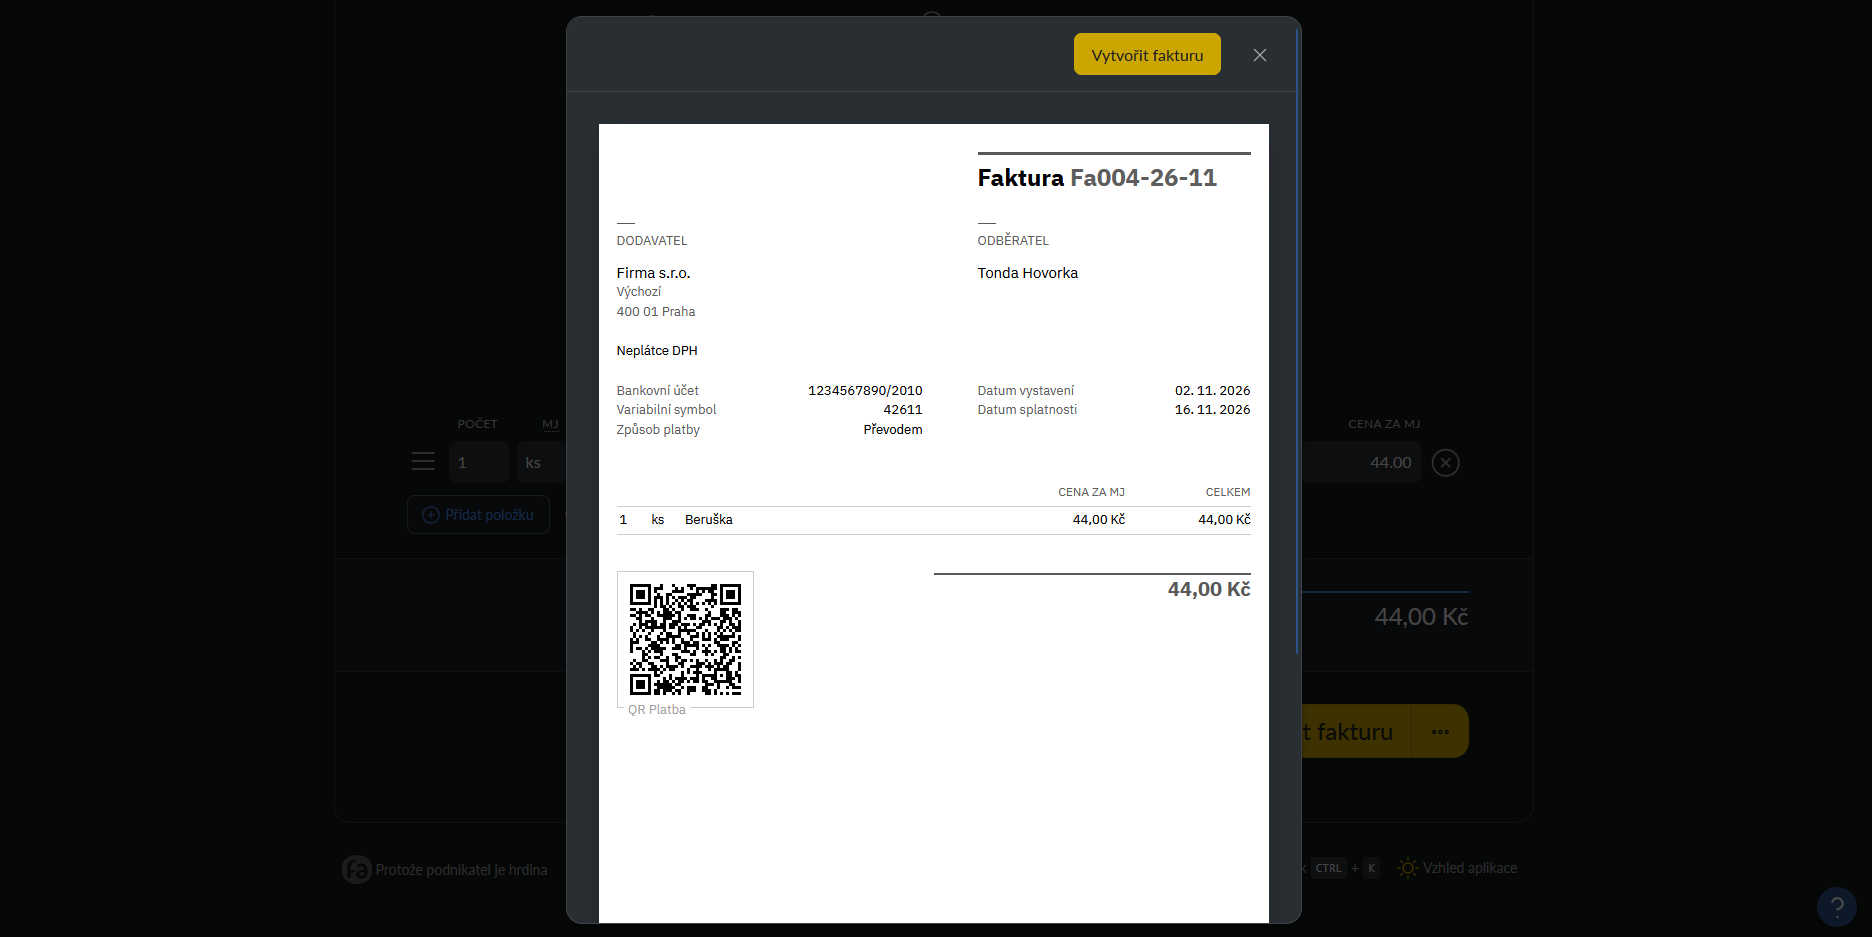
\includegraphics[width=0.85\linewidth]{obrazky/reserse/fakturoid_nahled_faktury.png}
\caption{Náhled faktury před jejím vystavením v~aplikaci Fakturoid (zdroj: vlastní snímek obrazovky ze zkušební verze, pořízeno 2.~11.~2026)}\label{obr:fakturoid-nahled}
\end{figure}

Řada prvků rozhraní je však nejasná. Cenové nabídky, šablony i~ceník jsou umístěny jako podzáložky v~sekci \emph{Faktury}. Šablony přitom neslouží ke změně vzhledu dokumentu, jak by název napovídal, ale k~uložení předvyplněné faktury pro opakované použití, a~pro nabídky nejsou k~dispozici vůbec. Vzhled dokumentu lze vybrat pouze ze šesti předdefinovaných variant. Po přechodu do ceníku se změní celá horní lišta a~uživatel ztratí přímý přístup k~fakturám a~nabídkám, aniž by mu rozhraní jasně ukázalo, ve které části aplikace se nachází. Stejné funkce jsou navíc dostupné z~více míst (z~tlačítka \enquote{+}, z~nabídky pod třemi tečkami a~z~hlavní navigace). Rušivě působí výrazná oznámení v~rámečku uprostřed obrazovky, která se zobrazují po každé akci, a~nápověda k~rychlým akcím, kterou se nepodařilo zavřít.

Přepsání čísla nabídky na vlastní tvar (například \texttt{NAB001-26}) formulář sice povolí, ale při uložení jej odmítne, protože neodpovídá formátu nastavenému pro číselnou řadu. Formát se nastavuje pomocí zástupných znaků, což je pro běžného uživatele zbytečně složité. Změnu jediného výchozího údaje, například splatnosti, nelze provést samostatně, ale jen přes celý formulář nastavení faktury. Nová ceníková položka se ve výchozím stavu zakládá jako skladová s~povinným množstvím, nákupní a~prodejní cenou, což servisní firma bez skladu nepotřebuje. Správa uživatelů a~oprávnění nebyla ve zkušební verzi dostupná.

Ve srovnání s~navrhovanou aplikací Fakturoid neobsahuje evidenci zakázek, zařízení ani provedené práce, materiál eviduje pouze formou skladu, neumožňuje vlastní šablony dokumentů a~místo kalendáře nabízí jen přehled a~statistiky. Cenové nabídky, sklad s~pohyby, upomínky a~více číselných řad jsou navíc dostupné až v~nejdražším tarifu \cite{fakturoid-srovnani}.

\subsection{Vhodnost pro malé firmy}

Fakturoid je velmi vhodný pro živnostníky a~malé firmy, které potřebují především rychle vystavovat faktury: nic se neinstaluje ani nespravuje, cena je nízká a~rozhraní přehledné. Servisní firma by však pokryla jen fakturační konec svého procesu a~evidenci zakázek by musela vést jinde. Data jsou uložena výhradně v~cloudu výrobce.

% Rešerše – iDoklad (vkládá se do kapitoly 01-reserse.tex)
\section{iDoklad}\label{sec:reserse-idoklad}

iDoklad je online fakturační a~evidenční služba ze skupiny, do které patří i~ekonomické systémy Money. Základní údaje shrnuje tabulka~\ref{tab:reserse-idoklad}.

\begin{table}[H]
\centering
\small
\begin{tabular}{>{\raggedright\arraybackslash}p{0.24\linewidth}>{\raggedright\arraybackslash}p{0.70\linewidth}}
\hline
\textbf{Kritérium} & \textbf{Zjištění} \\
\hline
Název & iDoklad \\
Společnost & Seyfor, a.s. (CZ; dříve Solitea) \cite{idoklad-web} \\
Typ aplikace & webová aplikace a~mobilní aplikace pro iOS a~Android \cite{idoklad-web,idoklad-vlastnosti} \\
Hostování & pouze cloud (SaaS provozovaný výrobcem); vlastní server ani lokální instalace nejsou možné \\
Licence & proprietární, předplatné \\
Cena & ceny bez DPH za měsíc při roční / čtvrtletní / měsíční platbě: Zdarma 0~Kč (1 uživatel, 5 kontaktů), Základní 187 / 220 / 240~Kč (2 uživatelé), Oblíbený 358 / 397 / 430~Kč (5 uživatelů), Prémiový 625 / 703 / 750~Kč (9 uživatelů) \cite{idoklad-cenik} \\
Zkušební verze & 60 dní v~tarifu Prémiový, bez platební karty; garance vrácení peněz do 30 dní \cite{idoklad-cenik,idoklad-vlastnosti} \\
\hline
\end{tabular}
\caption{Základní údaje o~řešení iDoklad}\label{tab:reserse-idoklad}
\end{table}

\subsection{Zkušenosti ze zkušební verze}

První dojem z~aplikace je velmi příjemný. Navigace je umístěna v~levém panelu s~ikonami, který lze zasunout a~získat tak více místa, což odpovídá návrhu navrhované aplikace. Výrazné zelené tlačítko \emph{Nový} umožňuje vytvořit libovolný doklad bez hledání v~záložkách. Tabulky faktur, nabídek i~ceníku vypadají jednotně, zobrazují jen potřebné sloupce a~další lze doplnit v~nastavení. Formulář cenové nabídky je totožný s~formulářem faktury, což usnadňuje orientaci. Sloupec se stavem dokladu přehledně ukazuje, v~jaké fázi se dokument nachází.

Formulář faktury zobrazuje poměrně mnoho údajů najednou, všechny však mají svůj smysl. Chybějící údaje jsou na rozdíl od Fakturoidu zobrazeny pouze jako varování ve spodní části formuláře a~doklad lze tlačítkem \emph{Přesto uložit} uložit i~s~nimi (obrázek~\ref{obr:idoklad-faktura}). Pořadové číslo dokladu lze změnit, formát číselné řady se ale nastavuje zástupnými znaky podobně jako ve Fakturoidu, i~když nápověda jejich význam vysvětluje. Tisk zobrazí náhled dokumentu, vzhled je však možné volit jen z~předdefinovaných variant a~funkce \emph{Šablony} slouží, stejně jako ve Fakturoidu, pouze k~předvyplnění opakovaných dokladů. Ceníkové položky stačí zadat jen názvem, ostatní údaje nejsou povinné. Velmi zdařilá jsou drobná vyskakovací oznámení, která jsou výrazná, ale nepřekážejí a~rychle zmizí, a~panel upozornění, který by v~navrhované aplikaci mohl sloužit pro upomínky blížících se termínů nebo historii posledních změn.

\begin{figure}[H]
\centering
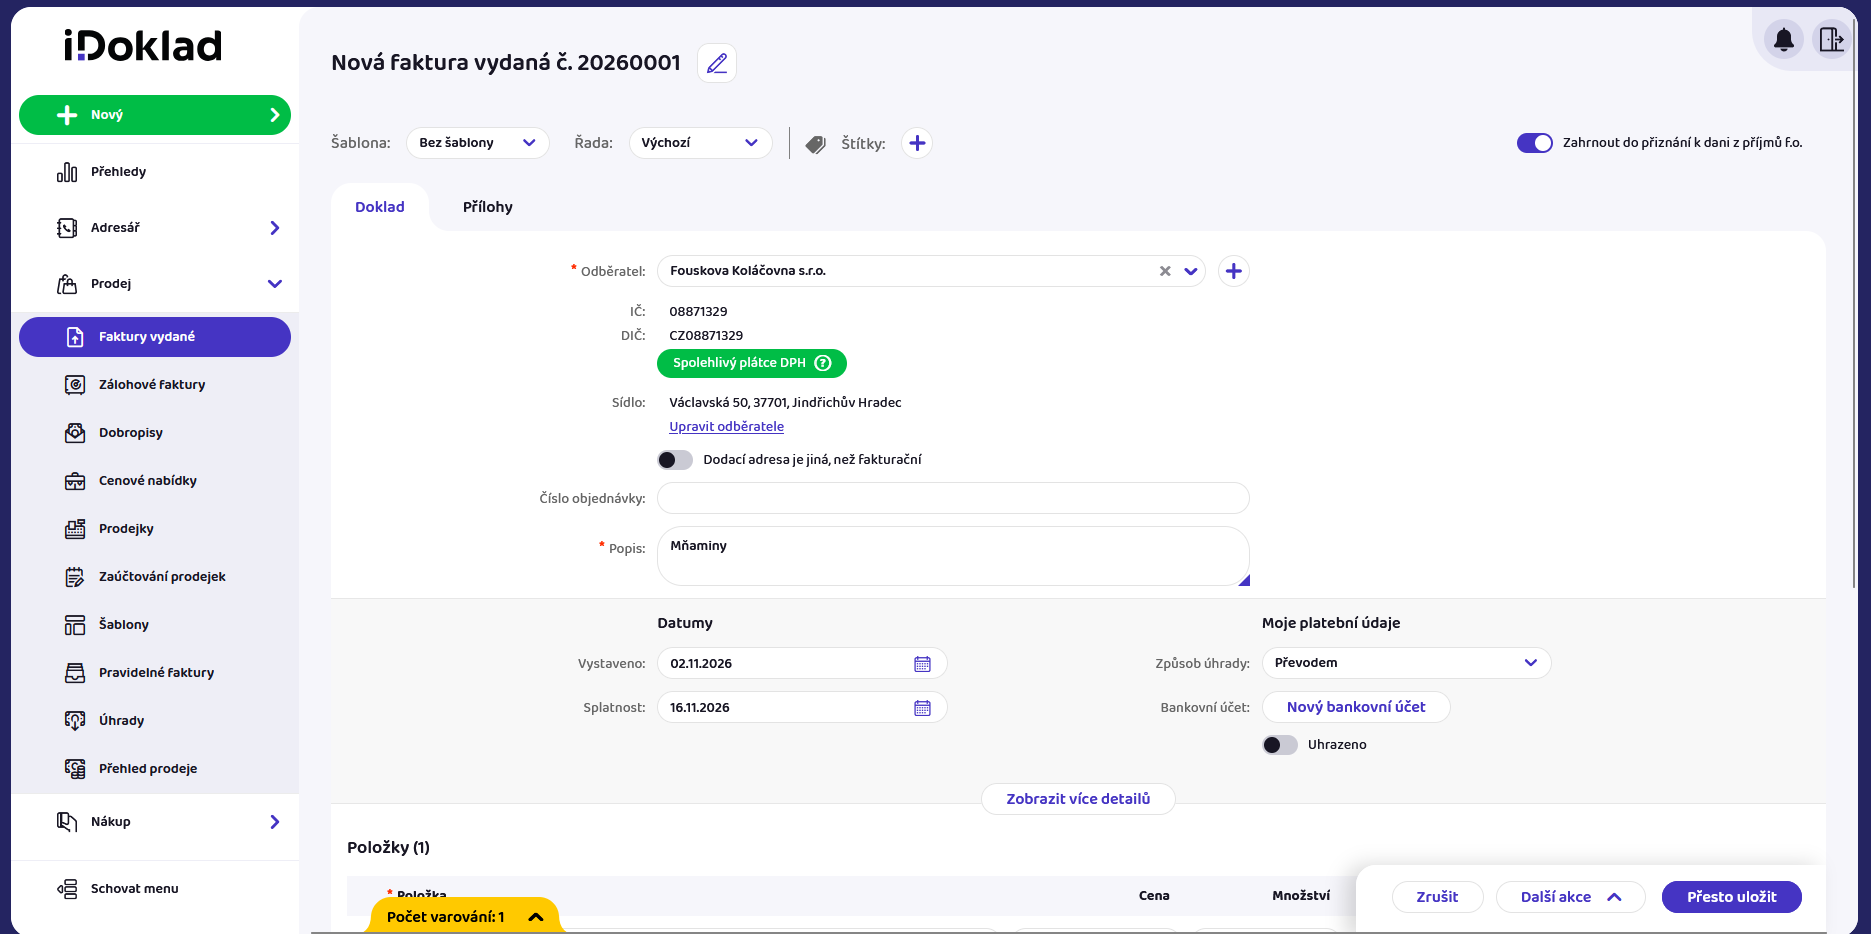
\includegraphics[width=\linewidth]{obrazky/reserse/iDoklad_tvorba_faktury.png}
\caption{Formulář nové faktury v~aplikaci iDoklad s~varováním o~chybějících údajích a~tlačítkem \emph{Přesto uložit} (zdroj: vlastní snímek obrazovky ze zkušební verze, pořízeno 2.~11.~2026)}\label{obr:idoklad-faktura}
\end{figure}

Nevýhodou je velké množství ikon s~akcemi přímo v~seznamu dokladů, z~nichž řada není pro běžnou práci potřeba a~stačila by v~detailu dokladu. Filtrování podle stavu (\emph{Všechny}, \emph{Uhrazené} atd.) je řešeno samostatnými položkami v~menu, přitom by stačil štítek se stavem u~každého dokladu a~filtr v~tabulce. Některé stránky nemají tlačítko \enquote{Zpět} a~ikona v~pravém horním rohu, která by jej mohla nahrazovat, uživatele odhlásí. Právě proto se navrhovaná aplikace drží doporučené zásady konzistence: tlačítka se stejným účelem mají na všech obrazovkách stejné umístění i~vzhled (oddíl~\ref{sec:ui-soulad}). Stejné nastavení seznamu je dostupné ze dvou různých tlačítek a~ve spodní části obrazovky se opakovaně zobrazuje propagace aplikace. Sekce Nákup (přijaté faktury, účtenky, Inbox) a~řada dokladů v~sekci Prodej (zálohové faktury, dobropisy, prodejky, pravidelné faktury) přesahují potřeby malé servisní firmy. Zajímavou inspirací pro možné rozšíření je naopak sekce Finance s~pokladnou pro evidenci hotovostních plateb.

Stejně jako Fakturoid je iDoklad primárně fakturační aplikace a~chybí v~něm evidence zakázek, zařízení, provedené práce a~kalendář.

\subsection{Vhodnost pro malé firmy}

iDoklad je vhodný pro živnostníky a~malé obchodní firmy, zejména pokud spolupracují s~externí účetní, která používá systémy Money nebo Pohoda \cite{idoklad-ucetni}. Jednotné a~přehledné rozhraní a~dlouhá zkušební doba usnadňují začátek. Pro servisní firmu ale pokryje opět jen fakturaci, data jsou uložena výhradně v~cloudu výrobce a~vyšší tarify jsou dražší než u~Fakturoidu.

% Rešerše – ABRA (vkládá se do kapitoly 01-reserse.tex)
\section{ABRA}\label{sec:reserse-abra}

Společnost ABRA Software nabízí dva produkty: ekonomický systém \emph{ABRA Flexi} (dříve FlexiBee) pro malé a~střední firmy a~ERP \emph{ABRA Aiva} pro střední a~velké firmy. Pro srovnání byla zvolena ABRA Flexi, která jako jediná nabízí zkušební verzi a~cílí na menší firmy. Základní údaje shrnuje tabulka~\ref{tab:reserse-abra}.

\begin{table}[H]
\centering
\small
\begin{tabular}{>{\raggedright\arraybackslash}p{0.24\linewidth}>{\raggedright\arraybackslash}p{0.70\linewidth}}
\hline
\textbf{Kritérium} & \textbf{Zjištění} \\
\hline
Název & ABRA Flexi (pro větší firmy ABRA Aiva) \\
Společnost & ABRA Software s.r.o., Praha (CZ); přibližně 35 let na trhu, přes 7~300 zákaznických firem \cite{abra-web} \\
Typ aplikace & webová aplikace a~desktopový klient pro Windows, Linux i~macOS \cite{abra-flexi-cenik} \\
Hostování & primárně cloud výrobce (Amazon Web Services); vlastní server je možný jen s~placenou rozšířenou podporou \cite{abra-flexi-cenik} \\
Licence & proprietární, předplatné bez vstupního poplatku \cite{abra-web} \\
Cena & za pojmenovaného uživatele a~měsíc při měsíční / roční platbě: Basic 425 / 390~Kč, Business 1~055 / 967~Kč, Premium 1~375 / 1~260~Kč; uživatelé pouze pro čtení zdarma; ABRA Aiva jen na poptávku, nasazení v~řádu stovek tisíc až milionů korun \cite{abra-flexi-cenik,abra-aiva-cena} \\
Zkušební verze & 30 dní všech tarifů, bez platební karty \cite{abra-flexi-cenik} \\
\hline
\end{tabular}
\caption{Základní údaje o~řešení ABRA}\label{tab:reserse-abra}
\end{table}

\subsection{Zkušenosti ze zkušební verze}

První dojem z~aplikace je velmi pozitivní, systém působí všestranně. Hned při založení účtu lze nastavit vzhled aplikace a~velikost písma, takže rozhraní je přehledné a~čitelné. Pro vyzkoušení si lze nechat vygenerovat ukázková data. Úvodní nástěnka zobrazuje souhrny a~grafy, které jsou příjemné, ale pro potřeby servisní firmy nejsou podstatné. Navigace je stejně jako u~iDokladu v~levém panelu, který lze zúžit jen na ikony. Modré tlačítko \emph{Nový} v~pravém horním rohu je dobře viditelné a~odlišené od ostatních prvků, formuláře mají v~pravém dolním rohu jednotná tlačítka \emph{Zavřít} a~\emph{Uložit a~zavřít}. Sekce \emph{Všechny agendy} umožňuje připnout si do menu jen potřebné části systému, což odpovídá myšlence navrhované aplikace, tedy funkčnímu jádru s~volitelnými rozšířeními.

Tabulky (adresář firem, vydané faktury) jsou jednotné a~přehledné, ale ve výchozím stavu zobrazují velké množství sloupců. Lze si nastavit zobrazené sloupce i~uložit vlastní pohledy, což je dobrý nápad, avšak pro malou firmu zbytečně složitý; po každé změně filtru či řazení navíc aplikace nabízí uložení pohledu. Filtrování se otevírá v~postranním panelu, který zbytek obrazovky zašedne. Detail záznamu se otevře jen kliknutím na sloupec \emph{Interní číslo}, nikoli na celý řádek, což není na první pohled patrné. Stav úhrady je zobrazen procentem zaplacené částky místo srozumitelného stavu (odesláno, zaplaceno). Inspirativní je naopak souhrn počtu dokladů a~jejich celkové částky ve spodní části tabulky. Formulář nové firmy obsahuje velké množství polí; pro potřeby servisní firmy by stačila základní část s~kontaktní osobou a~přílohami. Pozitivně lze hodnotit i~systém upozornění, který se zapíná v~nastavení a~nezakrývá obsah obrazovky. Globální vyhledávání v~horní části je naopak příliš obecné a~často vede do nastavení místo k~hledanému záznamu.

Zásadní rozdíl je v~pojetí zakázky (obrázek~\ref{obr:abra-zakazka}). Zakázka v~ABRA Flexi je chápána jako obchodní příležitost s~předpokládanými náklady a~ziskem, nikoli jako evidence přijatého zařízení a~průběhu opravy. Nabídky, objednávky a~zakázky jsou navíc dostupné až v~tarifu Business za 1~055~Kč za uživatele měsíčně. Tisk dokumentů nabízí výběr tiskové sestavy, možnost upravit vzhled dokumentu podle vlastní šablony se však v~uživatelském rozhraní nepodařilo najít, přestože nápověda popisuje konfigurovatelné reporty pro vybrané doklady \cite{abra-flexi-reporty}. Evidence zařízení, provedené práce a~kalendář v~systému chybí a~materiál je řešen pouze jako sklad.

\begin{figure}[H]
\centering
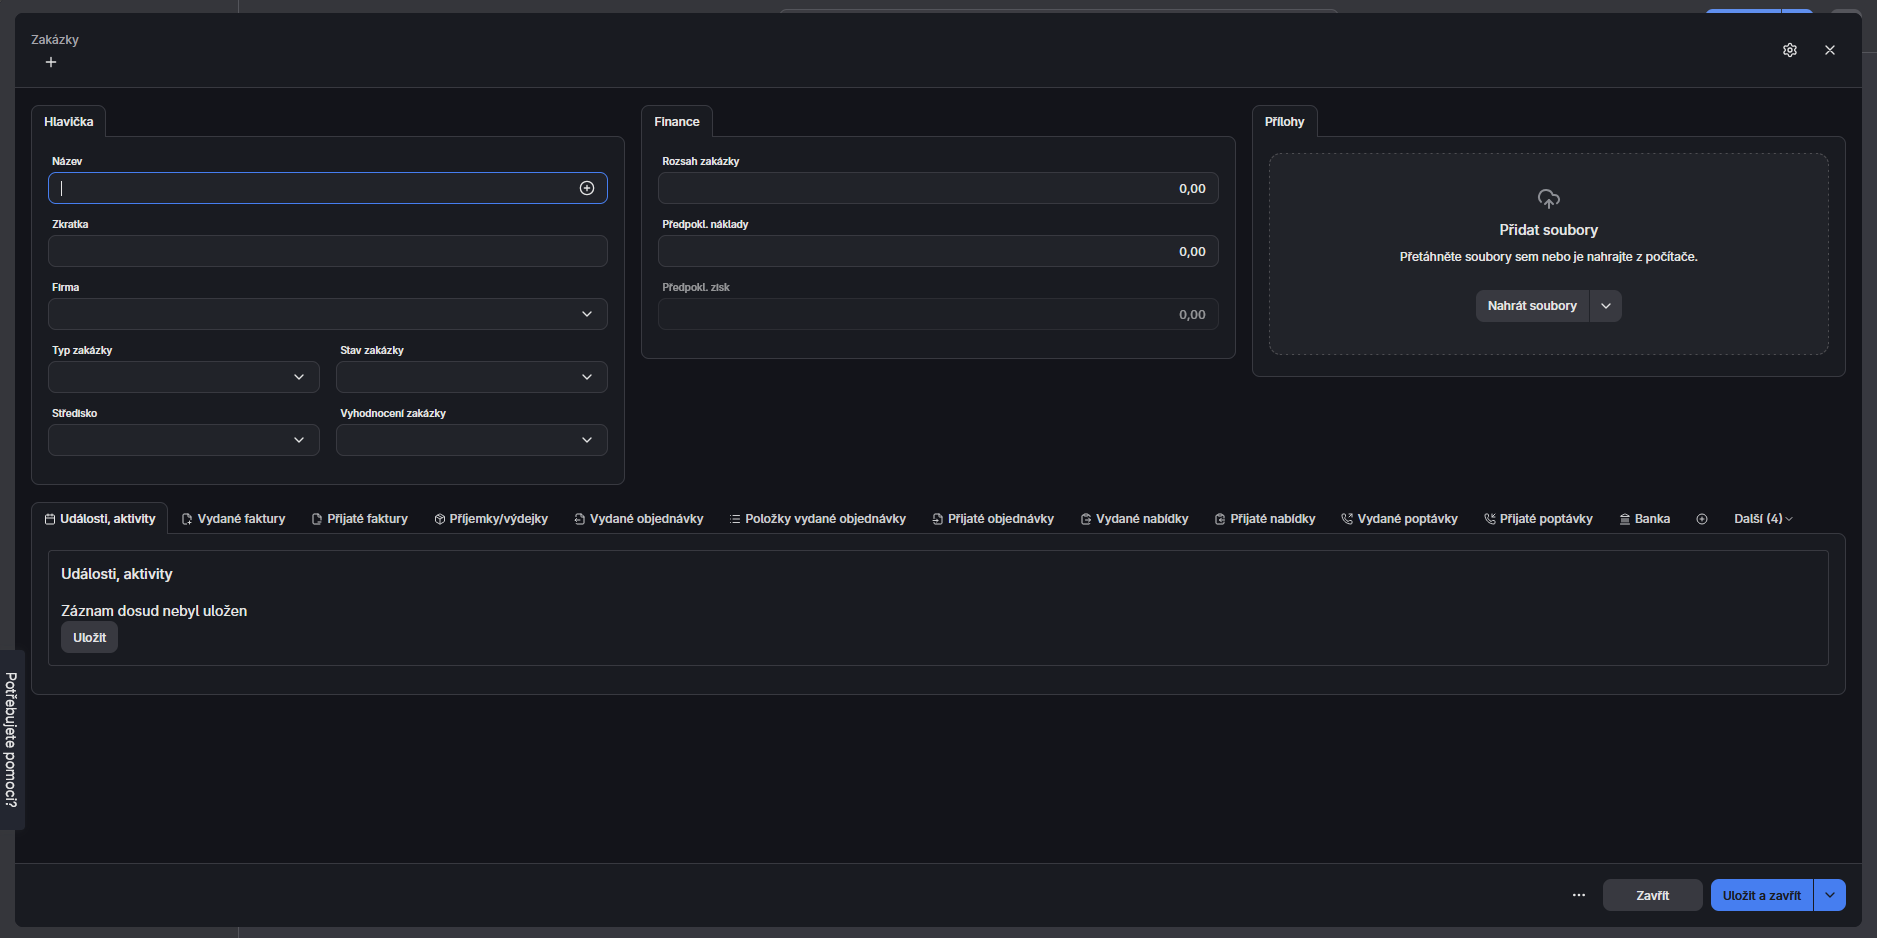
\includegraphics[width=\linewidth]{obrazky/reserse/abra_pridani_zakazky.png}
\caption{Formulář nové zakázky v~ABRA Flexi: zakázka je pojata jako obchodní případ s~rozsahem, náklady a~ziskem (zdroj: vlastní snímek obrazovky ze zkušební verze, pořízeno 3.~11.~2026)}\label{obr:abra-zakazka}
\end{figure}

\subsection{Vhodnost pro malé firmy}

ABRA Flexi je vhodná pro malé firmy, které chtějí vést kompletní účetnictví a~daňovou evidenci samy. Pro malou servisní firmu však nemá přiměřený poměr ceny a~přínosu: tarif Basic obsahuje z~potřebných funkcí v~podstatě jen fakturaci, kterou levněji nabízejí fakturační nástroje, a~tarif Business, který se potřebám firmy blíží nejvíce, stojí přes 1~000~Kč za uživatele měsíčně, a~přesto neobsahuje servisní evidenci. Rozhraní je přehledné a~přizpůsobitelné, ale orientované na zkušené administrativní a~účetní pracovníky.

% Rešerše – ERPNext (vkládá se do kapitoly 01-reserse.tex)
\section{ERPNext}\label{sec:reserse-erpnext}

ERPNext je open-source podnikový systém postavený na frameworku Frappe v~jazyce Python. Základní údaje shrnuje tabulka~\ref{tab:reserse-erpnext}.

\begin{table}[H]
\centering
\small
\begin{tabular}{>{\raggedright\arraybackslash}p{0.24\linewidth}>{\raggedright\arraybackslash}p{0.70\linewidth}}
\hline
\textbf{Kritérium} & \textbf{Zjištění} \\
\hline
Název & ERPNext \\
Společnost & Frappe Technologies Pvt. Ltd. (Indie) a~komunita; první verze v~roce 2010 \cite{wiki-erpnext} \\
Typ aplikace & webová aplikace (Python, framework Frappe, databáze MariaDB) \cite{wiki-erpnext,erpnext-web} \\
Hostování & vlastní server zdarma, nebo cloud Frappe Cloud \cite{erpnext-cenik} \\
Licence & open-source, GNU GPL v3; žádné funkce nejsou zpoplatněny \cite{erpnext-github,erpnext-web} \\
Cena & software zdarma; Frappe Cloud se neplatí za uživatele, ale podle výkonu: sdílený hosting od 5~USD, vlastní server od 20~USD měsíčně \cite{erpnext-cenik} \\
Zkušební verze & 14 dní na Frappe Cloud \cite{erpnext-cenik} \\
\hline
\end{tabular}
\caption{Základní údaje o~řešení ERPNext}\label{tab:reserse-erpnext}
\end{table}

\subsection{Zkušenosti ze zkušební verze}

Průvodce prvním nastavením se zobrazil v~angličtině a~aplikace byla proto hodnocena v~anglickém prostředí. Projekt sice obsahuje komunitní český překlad rozhraní \cite{erpnext-github}, oficiální česká lokalizace (například podpora formátu ISDOC nebo českých daňových výkazů) však neexistuje \cite{frappe-forum-cz}.

Rozhraní působí minimalisticky a~přehledně: v~levé části je lišta s~ikonami modulů, jejichž název se zobrazí po najetí myší, a~vedle ní seznam podkategorií. Sekce \emph{Setup} nabízí velké množství možností, od správy uživatelů, organizace a~přístupových rolí po nastavení tiskových dokumentů, včetně úpravy hlavičky dokumentu v~jazyce HTML. Všechny volby jsou přehledné a~tlačítka pro uložení nebo přidání záznamu jasně viditelná, celkově však aplikace působí jako nástroj pro zkušeného administrátora, který si systém sám nastaví, nikoli pro běžného zaměstnance malé firmy. Bez zaškolení by úvodní nastavení zabralo několik hodin. Příjemně jednoduché je založení nového uživatele, kde stačí vyplnit e-mail a~jméno, s~možností zobrazit celý formulář. Panel upozornění je funkční (všechna upozornění nebo jen nadcházející události), ale zobrazuje se přes celou výšku stránky a~zakrývá obsah (obrázek~\ref{obr:erpnext-upozorneni}). Evidence zakázek je vedena prostřednictvím projektů, takže každá servisní zakázka by musela být založena jako samostatný projekt, což je pro servisní praxi zbytečná administrativní zátěž.

\begin{figure}[H]
\centering
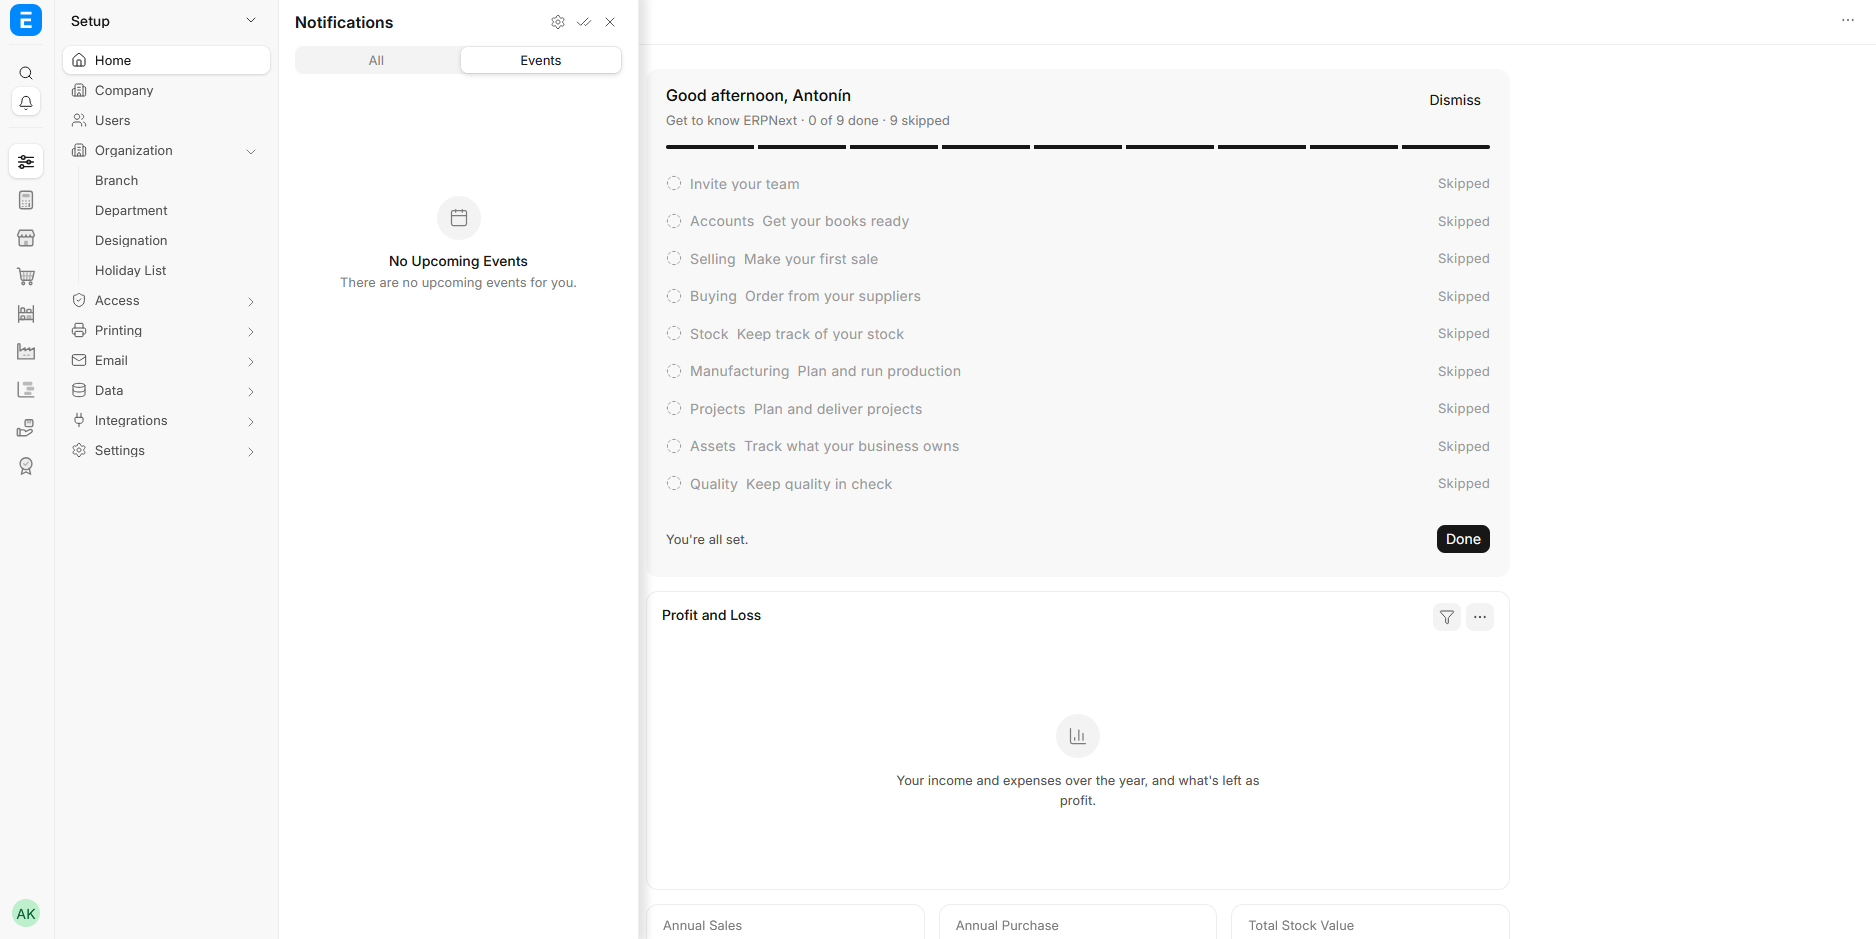
\includegraphics[width=\linewidth]{obrazky/reserse/erpnext_upozorneni.png}
\caption{Panel upozornění v~ERPNext zobrazený přes celou výšku stránky (zdroj: vlastní snímek obrazovky ze zkušební verze, pořízeno 3.~11.~2026)}\label{obr:erpnext-upozorneni}
\end{figure}

\subsection{Vhodnost pro malé firmy}

Cenově je ERPNext pro malou firmu velmi vhodný: software je zdarma a~cloudový provoz se neplatí za uživatele. Překážkou je však chybějící česká lokalizace, nedostatek implementačních partnerů v~České republice a~náročnost nastavení i~vlastního provozu, který vyžaduje znalost Linuxu, Pythonu a~databáze MariaDB. Pro malou servisní firmu bez technického zázemí je proto nasazení obtížné. Architekturou, tedy open-source webovou aplikací v~jazyce Python, je však ze všech srovnávaných řešení navrhované aplikaci nejblíže.

% Rešerše – Odoo (vkládá se do kapitoly 01-reserse.tex)
\section{Odoo}\label{sec:reserse-odoo}

Odoo je modulární podnikový systém složený z~desítek aplikací, ze kterých si firma vybírá jen ty, které potřebuje. Základní údaje shrnuje tabulka~\ref{tab:reserse-odoo}.

\begin{table}[H]
\centering
\small
\begin{tabular}{>{\raggedright\arraybackslash}p{0.24\linewidth}>{\raggedright\arraybackslash}p{0.70\linewidth}}
\hline
\textbf{Kritérium} & \textbf{Zjištění} \\
\hline
Název & Odoo (dříve TinyERP a~OpenERP) \\
Společnost & Odoo S.A., Belgie; zakladatel a~generální ředitel Fabien Pinckaers \cite{wiki-odoo,odoo-zdrazeni} \\
Typ aplikace & webová aplikace a~mobilní aplikace \\
Hostování & cloud výrobce (Odoo Online), platforma Odoo.sh i~vlastní server \cite{wiki-odoo,odoo-cenik} \\
Licence & dvě edice: Community jako open-source (LGPLv3), Enterprise jako proprietární předplatné \cite{wiki-odoo,odoo-github} \\
Cena & Community zdarma; v~cloudu je jedna aplikace zdarma s~neomezeným počtem uživatelů; tarif Standardní 11,90~€ (běžně 14,90~€) a~Nestandardní 22,90~€ (běžně 27,90~€) za uživatele a~měsíc; vlastní server, úpravy přes Odoo Studio a~API jen v~tarifu Nestandardní (obrázek~\ref{obr:odoo-cenik}) \cite{odoo-cenik}; implementace u~českých partnerů pro malou firmu přibližně 150 až 400 tisíc~Kč \cite{elfox-odoo} \\
Zkušební verze & 15 dní pro více aplikací, jedna aplikace je zdarma trvale \cite{odoo-cenik} \\
\hline
\end{tabular}
\caption{Základní údaje o~řešení Odoo}\label{tab:reserse-odoo}
\end{table}

\begin{figure}[H]
\centering
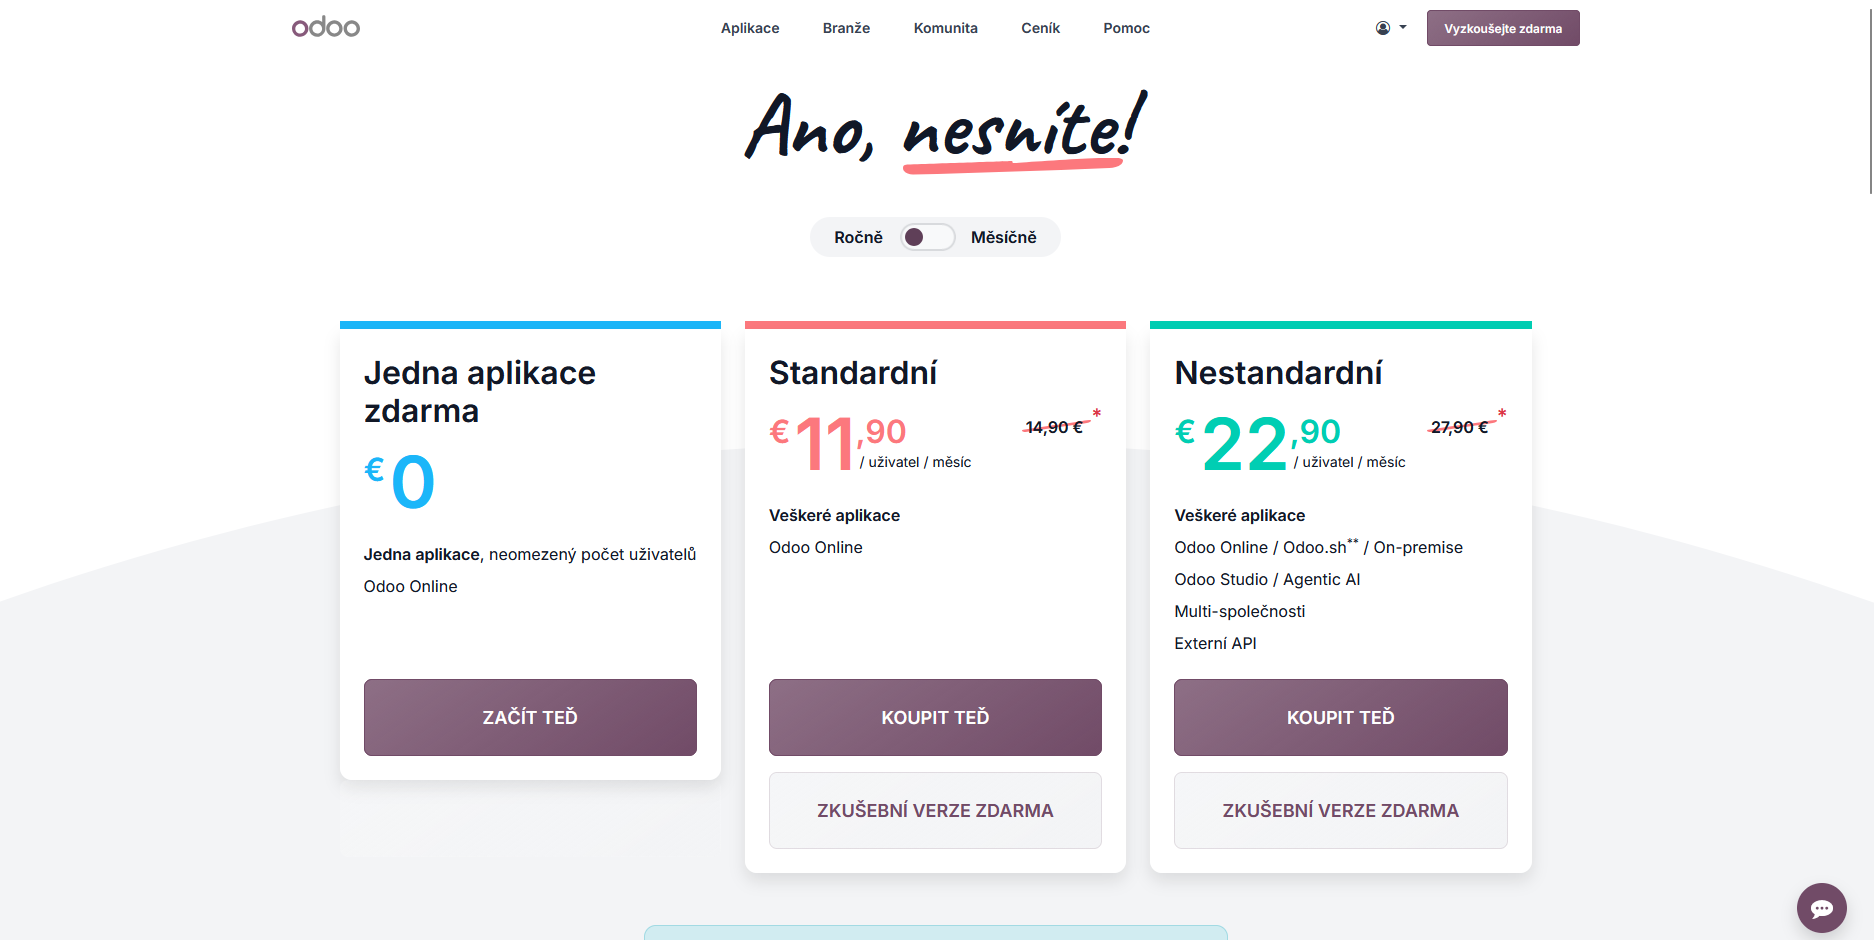
\includegraphics[width=0.9\linewidth]{obrazky/reserse/odoo_cenik_predplatne.png}
\caption{Ceník Odoo pro Českou republiku (zdroj: vlastní snímek obrazovky stránky \protect\url{https://www.odoo.com/cs_CZ/pricing}, pořízeno 3.~11.~2026)}\label{obr:odoo-cenik}
\end{figure}

\subsection{Zkušenosti ze zkušební verze}

Ve zkušební verzi byly vybrány aplikace CRM, Pokladní systém, Fakturace, Dokumenty, Opravy a~Zaměstnanci. Odoo bylo vyzkoušeno jako poslední, protože od něj byl na základě předchozí rešerše očekáván největší přínos. Úvodní obrazovka působí přívětivě: barevné ikony jednotlivých aplikací na tmavém pozadí s~názvy, název firmy a~přihlášený uživatel v~pravém horním rohu. Důležitá tlačítka, například \emph{Nové}, jsou barevně odlišená a~horní lišta ukazuje, ve které části aplikace se uživatel nachází. Tabulky jsou přehledné a~lze je přepnout do zobrazení kanban, seznam, graf nebo kalendář; kanbanové zobrazení kontaktů s~kartami obsahujícími jen základní údaje je velmi přehledné a~je inspirací pro navrhovanou aplikaci. Formulář nového kontaktu má vlevo vstupní pole a~vpravo souhrnný přehled, podobně jako v~navrhované aplikaci, záznam se však ukládá automaticky bez tlačítka \emph{Uložit}, takže uživatel nemá jistotu, zda byl uložen. Stránka Dokumenty se stromem složek je přehledná a~usnadňuje hledání v~uložených souborech. Příjemná je také sekce Aplikace, kde lze aplikace kdykoliv přidat nebo odebrat.

Aplikace Opravy umožňuje založit opravu výrobku i~nový výrobek přímo z~formuláře (obrázek~\ref{obr:odoo-opravy}). Stavy opravy jsou ale jen tři (\emph{Nové}, \emph{Potvrzený} a~\emph{Done}), částečně nepřeložené. Po dokončení opravy lze tlačítkem \emph{Invoice} vytvořit fakturu. Detail faktury nabízí akce Odeslat, Tisk, Zaplatit a~Náhled; tisk však bez náhledu rovnou stáhne soubor PDF a~po jednorázovém výběru vzhledu dokumentu (\emph{Setup your invoice layout}) se možnost jej znovu změnit nepodařilo najít. Nastavit formát číslování dokumentů nelze.

\begin{figure}[H]
\centering
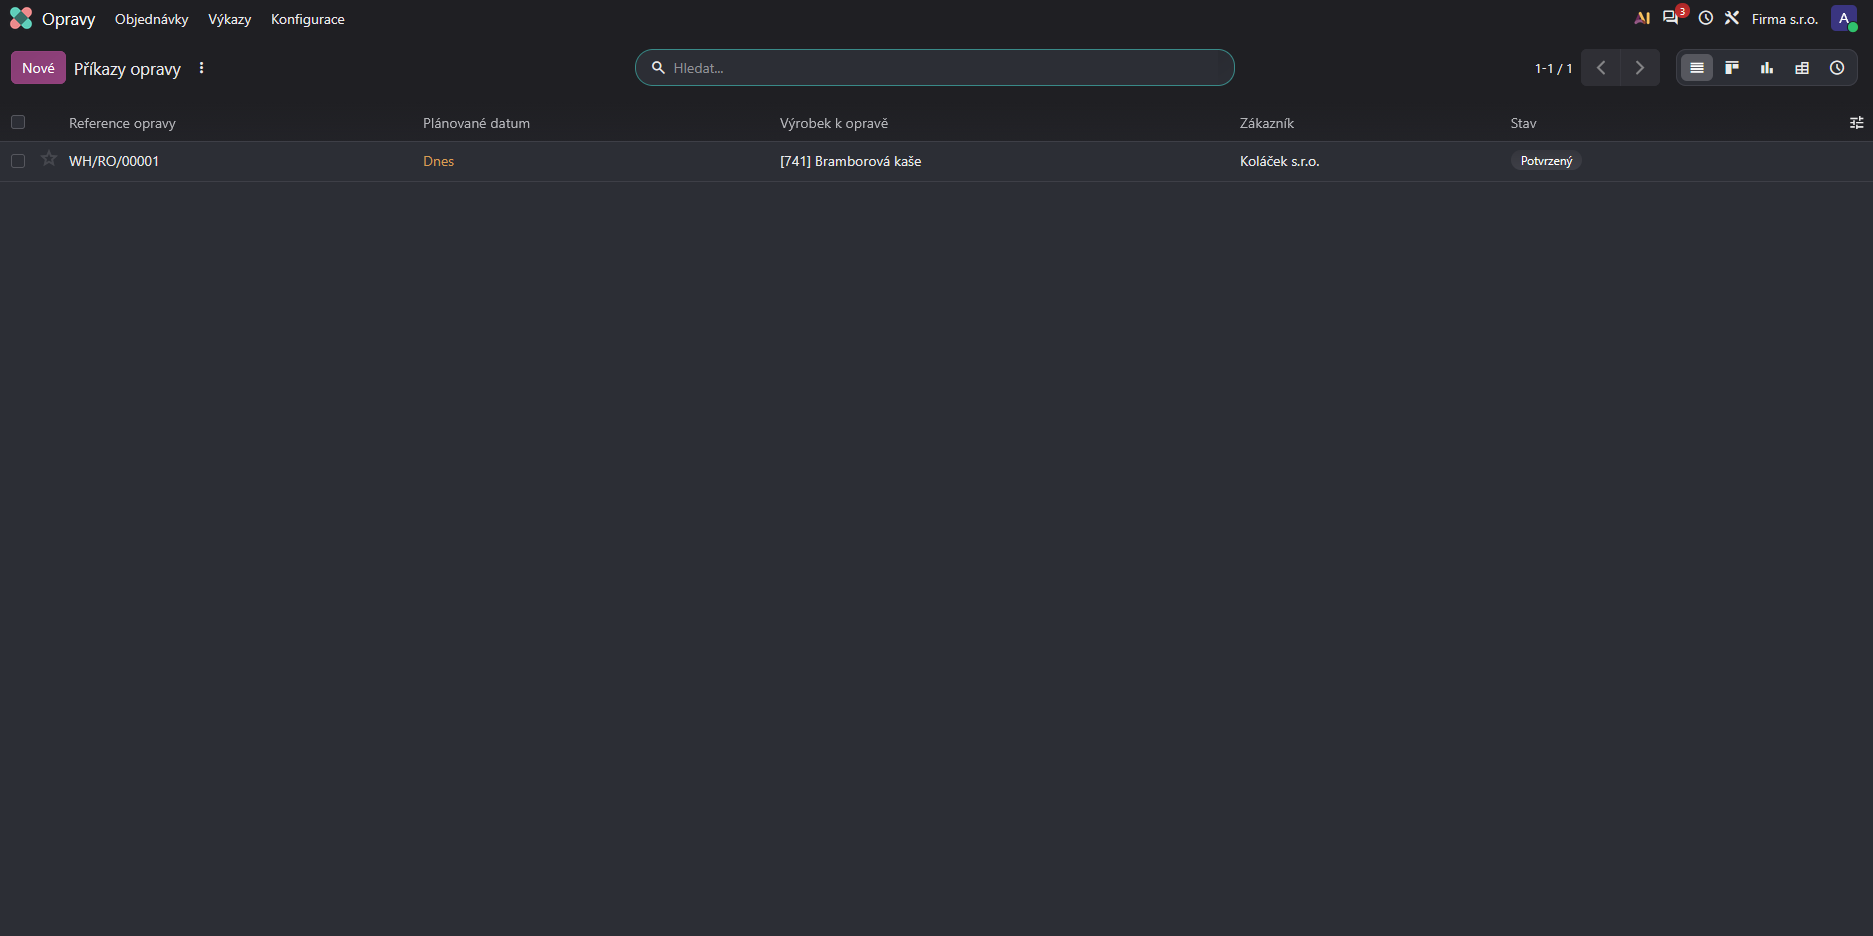
\includegraphics[width=\linewidth]{obrazky/reserse/odoo_strana_opravy.png}
\caption{Seznam oprav v~aplikaci Odoo s~přepínáním zobrazení vpravo nahoře (zdroj: vlastní snímek obrazovky ze zkušební verze, pořízeno 3.~11.~2026)}\label{obr:odoo-opravy}
\end{figure}

Celkový dojem je přesto zklamáním. Navigace je nelogická: odkazy jako \emph{Objednávky} v~aplikaci Opravy vedou na tutéž stránku, \emph{Výkazy} zobrazí jen graf, nabídky jsou skryté pod položkou \emph{Objednávky} a~položky \emph{Zákazníci} a~\emph{Dodavatelé} v~aplikaci Fakturace pouze otevírají další nabídku, takže k~vytvoření faktury vede několik nepřímých kroků. Rozhraní je přeloženo jen částečně, anglické texty se objevují v~tlačítkách i~vstupních polích. Popisky ikon pro přepínání zobrazení se zobrazují pod kurzorem, který je zakrývá. Pravou část každého formuláře zabírá panel s~chatem, historií změn a~aktivitami určený pro spolupráci více zaměstnanců; zabírá téměř polovinu obrazovky, nelze změnit jeho velikost a~pro firmu s~jedním administrativním pracovníkem je zbytečný. Tlačítka \emph{Zrušit} a~\emph{Uložit} v~nastavení bez provedených změn nedělají nic viditelného, chybí tlačítko \enquote{Zpět} (nahrazuje jej jen malý křížek) a~po výběru sekce se nejprve zobrazí přehled s~grafy. Ve srovnání s~navrhovanou aplikací chybí evidence zařízení (aplikace Opravy tento požadavek nesplňuje), servisních zakázek a~provedené práce, materiál je dostupný jen jako součást skladu a~nelze použít vlastní šablony dokumentů.

\subsection{Vhodnost pro malé firmy}

Pokud by firma řešila pouze fakturaci, je Odoo díky trvale bezplatné jedné aplikaci výhodnější než placené fakturační služby. Pro pokrytí potřeb servisní firmy by však musela používat více aplikací v~placeném tarifu za přibližně 12~€ za uživatele měsíčně, a~ani tak by servisní evidence neodpovídala jejím požadavkům. Edice Community je zdarma, ale její provoz na vlastním serveru vyžaduje technické znalosti a~implementace u~partnera se pohybuje ve stovkách tisíc korun. Odoo je tak funkčně silné, ale pro malou servisní firmu provozně i~ekonomicky náročné a~vhodné spíše pro firmy, které počítají s~růstem.

% Rešerše – HELIOS (vkládá se do kapitoly 01-reserse.tex)
\section{HELIOS}\label{sec:reserse-helios}

Informační systémy HELIOS tvoří produktovou řadu od HELIOS Red pro živnostníky přes HELIOS Easy pro malé firmy a~HELIOS iNuvio pro malé a~střední firmy po HELIOS Nephrite pro velké firmy \cite{autoerp-srovnani}. Pro srovnání byl zvolen HELIOS iNuvio, nástupce rozšířeného systému HELIOS Orange. Základní údaje shrnuje tabulka~\ref{tab:reserse-helios}.

\begin{table}[H]
\centering
\small
\begin{tabular}{>{\raggedright\arraybackslash}p{0.24\linewidth}>{\raggedright\arraybackslash}p{0.70\linewidth}}
\hline
\textbf{Kritérium} & \textbf{Zjištění} \\
\hline
Název & HELIOS iNuvio (řada HELIOS Red, Easy, iNuvio, Nephrite) \\
Společnost & Asseco Solutions, a.s., Praha (CZ); přes 15~000 zákazníků \cite{helios-fenix-pl} \\
Typ aplikace & desktopová aplikace pro Windows v~architektuře klient--server nad databází Microsoft SQL Server \cite{helios-pozadavky} \\
Hostování & vlastní server nebo jediný počítač, vzdálený přístup přes vzdálenou plochu; cloud jako samostatná služba výrobce nebo u~partnerů \cite{helios-pozadavky,helios-inuvio,appon-inuvio} \\
Licence & proprietární \\
Cena & nezveřejněna, stanovuje se individuálně po analýze potřeb firmy; implementace trvá měsíce \cite{helios-inuvio,autoerp-srovnani} \\
Zkušební verze & není, pouze předváděcí demo na vyžádání \cite{helios-inuvio} \\
\hline
\end{tabular}
\caption{Základní údaje o~řešení HELIOS}\label{tab:reserse-helios}
\end{table}

\subsection{Zhodnocení}

HELIOS nenabízí zkušební verzi ani interaktivní ukázku, a~uživatelské rozhraní proto nebylo možné vlastnoručně vyzkoušet. Potenciální zákazník nemá možnost ověřit, zda systém odpovídá jeho potřebám, aniž by kontaktoval obchodní oddělení výrobce. Podle výrobce obsahuje HELIOS iNuvio ekonomiku, sklady, obchod s~CRM, lidské zdroje, výrobu, dopravu a~modul řízení projektů a~servisu \cite{helios-inuvio}, k~dispozici je otevřené API a~napojení na registr ARES \cite{ucetnictvi-inuvio}. Podrobný popis servisních funkcí však výrobce veřejně nezveřejňuje.

\subsection{Vhodnost pro malé firmy}

Pro malou firmu je HELIOS iNuvio málo vhodný. Vyžaduje vlastní server s~operačním systémem Windows nebo placený hosting, licence a~implementaci na míru, a~neveřejná cena spolu s~chybějící zkušební verzí brání rychlému rozhodnutí. Systém je určen středním a~větším firmám se složitými procesy, jako je výroba, rozsáhlé sklady nebo mzdy.


\section{Souhrnné srovnání}\label{sec:reserse-srovnani}

Tabulka~\ref{tab:reserse-souhrn} shrnuje základní charakteristiky všech srovnávaných řešení. Pro úplnost je v~ní uvedena i~navrhovaná aplikace BusinessManager.

\begin{table}[htbp]
\centering
\footnotesize
\setlength{\tabcolsep}{3pt}
\resizebox{\textwidth}{!}{%
\begin{tabular}{>{\raggedright\arraybackslash}p{2.0cm}>{\raggedright\arraybackslash}p{2.4cm}>{\raggedright\arraybackslash}p{1.5cm}>{\raggedright\arraybackslash}p{2.3cm}>{\raggedright\arraybackslash}p{1.9cm}>{\raggedright\arraybackslash}p{2.7cm}>{\raggedright\arraybackslash}p{1.8cm}}
\hline
\textbf{Řešení} & \textbf{Společnost} & \textbf{Typ} & \textbf{Hostování} & \textbf{Licence} & \textbf{Cena (měsíčně)} & \textbf{Vhodnost pro malou firmu} \\
\hline
Fakturoid & Fakturoid s.r.o. (CZ) & web, mobil & cloud & proprietární & 0--519 Kč s DPH & vysoká (jen fakturace) \\
iDoklad & Seyfor, a.s. (CZ) & web, mobil & cloud & proprietární & 0--750 Kč bez DPH & vysoká (jen fakturace) \\
ABRA Flexi & ABRA Software s.r.o. (CZ) & web, desktop & cloud (vlastní server s příplatkem) & proprietární & 390--1 375 Kč za uživatele & střední \\
ERPNext & Frappe Technologies (IN) & web & cloud i vlastní server & GPLv3 & zdarma;\newline cloud od 5~USD & střední (bez české lokalizace) \\
Odoo & Odoo S.A. (BE) & web, mobil & cloud i vlastní server & LGPLv3 / proprietární & jedna aplikace zdarma; 11,90--22,90 € za uživatele & střední \\
HELIOS iNuvio & Asseco Solutions, a.s. (CZ) & desktop (Windows) & vlastní server, cloud u partnerů & proprietární & na poptávku & nízká \\
\hline
Business\-Manager & vlastní řešení & web & vlastní server / lokální PC & open-source & zdarma & cílové řešení \\
\hline
\end{tabular}}
\caption{Souhrnné srovnání základních charakteristik řešení}\label{tab:reserse-souhrn}
\end{table}

Ze srovnání vyplývá, že řešení se dělí do dvou skupin. Fakturační nástroje Fakturoid a~iDoklad jsou levné, přehledné a~mají vyřešenou českou legislativu, nepokrývají však servisní část procesu: evidenci zařízení, zakázek, provedené práce ani kalendář. Podnikové systémy ABRA, ERPNext, Odoo a~HELIOS některé z~těchto oblastí obsahují, ale za cenu složitého rozhraní, nutnosti delšího zaškolení a~u~proprietárních řešení i~vyšších nákladů. Pojem zakázky navíc tyto systémy chápou jinak než servisní firma: ABRA jako obchodní příležitost, ERPNext jako projekt a~Odoo jako opravu výrobku s~velmi jednoduchými stavy. Žádné ze srovnávaných řešení tak nespojuje evidenci servisních zakázek a~zařízení, tvorbu dokumentů podle vlastních šablon, podporu formátu ISDOC, jednoduché rozhraní a~bezplatný provoz na vlastním počítači či serveru. Tato mezera je hlavním důvodem pro vývoj vlastní aplikace.

\section{Inspirace pro návrh aplikace}\label{sec:reserse-inspirace}

Rešerše přinesla řadu podnětů, které byly při návrhu aplikace využity, nebo jsou zaznamenány jako možná rozšíření:
\begin{itemize}
\item \textbf{Náhled dokumentu před jeho vytvořením} (Fakturoid, obrázek~\ref{obr:fakturoid-nahled}). Na rozdíl od Fakturoidu však aplikace náhled neblokuje kvůli nevyplněným údajům, pouze na ně upozorní.
\item \textbf{Upozornění místo blokování} (iDoklad, obrázek~\ref{obr:idoklad-faktura}): chybějící údaje jsou zobrazeny jako varování a~dokument lze přesto uložit. Podobně má aplikace upozornit na nevyplněné údaje o~firmě po první instalaci.
\item \textbf{Soukromá poznámka} k~dokladu (Fakturoid), oddělená od textu určeného zákazníkovi, například pro poznámky o~potřebném materiálu.
\item \textbf{Upozornění a~upomínky} (iDoklad, ABRA): přehled událostí, které je třeba vyřešit, například blížící se splatnost faktur nebo naposledy vytvořené dokumenty, aby další pracovník věděl, kde předchozí den skončila práce. V~aplikaci mohou vycházet z~části Kalendář.
\item \textbf{Souhrn počtu a~celkové částky dokladů} pod tabulkou (ABRA), zobrazovaný jen uživatelům s~oprávněním vidět finanční údaje; využití popisuje oddíl~\ref{sec:ui-inspirace}.
\item \textbf{Kanbanové zobrazení} zákazníků, zařízení či zakázek jako alternativa k~tabulce (Odoo); využití popisuje oddíl~\ref{sec:ui-inspirace}.
\item \textbf{Číslování dokumentů podle vzoru}: formát čísla se zadá ukázkou, například \texttt{NAB001-26}, místo složitého zápisu se zástupnými znaky, jaký používají Fakturoid a~iDoklad.
\item \textbf{Pokladna} pro evidenci hotovostních plateb (iDoklad) jako možný rozšiřující modul.
\end{itemize}
Naopak jako odstrašující příklady posloužily výrazná vyskakovací upozornění uprostřed obrazovky, zdvojené ovládací prvky se stejnou funkcí, chybějící tlačítko \enquote{Zpět} a~nejednotný jazyk rozhraní.
